% !Mode:: "TeX:UTF-8"

\chapter{表格、图片和公式的使用}
\section{表格}
论文中的表格一般使用三线表进行绘制,以下使用tabular环境举例。\par
表 \ref{student_info} 是一个简单的例子。 \par
\begin{table}
\zihao{5}
\label{student_info}
\begin{center}
\caption{学生信息}
\begin{tabular}{ccc}
    \toprule
    学号  &   姓名  &   班级\\
    \midrule
    b20150001   &   张三  &   一班\\
    b20150002   &   李四  &   二班\\
    b20150003   &   王五  &   三班\\
    \bottomrule
\end{tabular}
\end{center}
\end{table}

表\ref{student_info2}是一个多行多列表格的例子。 \par
\begin{table}
\caption{学生信息2}
\label{student_info2}
\begin{center}
\begin{tabular}{cccc}
    \hline
    \multirow{2}{*}{学号}  &  \multirow{2}{*}{姓名}  &   \multicolumn{2}{c}{联系方式}\\
        &   &   Email   &   手机号\\
    \hline
    b20150001   &   张三  &   12345678@qq.com &   13811110001\\
    b20150002   &   李四  &       &   13912345678\\
    b20150003   &   王五  &   helloworld@gmail.com    &   \\
    \hline
\end{tabular}
\end{center}
\end{table}


\section{图片}
插入图片有两种情况,一种是插入位图,一种是插入矢量图。比如要插入数学图像和图表,假如从 Mathematica 软件中导出图片时,记得保存为 pdf 或 eps,它们是矢量格式,插图后不会模糊。无论在\LaTeX 插入什么图片,都需要在导言区导入宏包usepackage{graphics},\LaTeX 最有名的就是支持eps ( Encapsulated PostScript )格式的图片的插入,不过\LaTeX 对图形插入的格式进行了扩展,比如支持插入pdf格式的图片,需要在导言区插入$\backslash$usepackage \{graphicx\},一般使用$\backslash$usepackage\{graphicx\} 就能对graphics进行支持。不过需要注意的是插入eps 格式的图片时,必须使用 latex 和 dvipdf 两个命令,在编辑器 WinEdt 中有两个按钮;而插入pdf格式的图片时,使用的命令就是pdflatex了,它可以直接将源文件*.tex编译生成*.pdf文件。 \par
在\LaTeX 中,对于双栏格式的排版,插入一栏图片时,使用的是$\backslash$begin\{figure\} …… $\backslash$end\{figure\} , 插入双栏图片时需在figure的上标中加入符号“*”,如$\backslash$begin\{figure*\} …… $\backslash$end\{figure*\}。\par
\subsection{插入一张图片}
在latex插入一张图片(占一栏)比较简单,图\ref{fig_example1}为插入一张图片例子。如果插入eps格式的图片需要使用LaTeX 进行编译,不能使用PdfTeXify编译;如果插入png、jpg格式的图片则需要使用PdfTeXify 进行编译,不能使用LaTeX 编译。\par
\begin{figure}
\centering      %使插入的图片居中显示
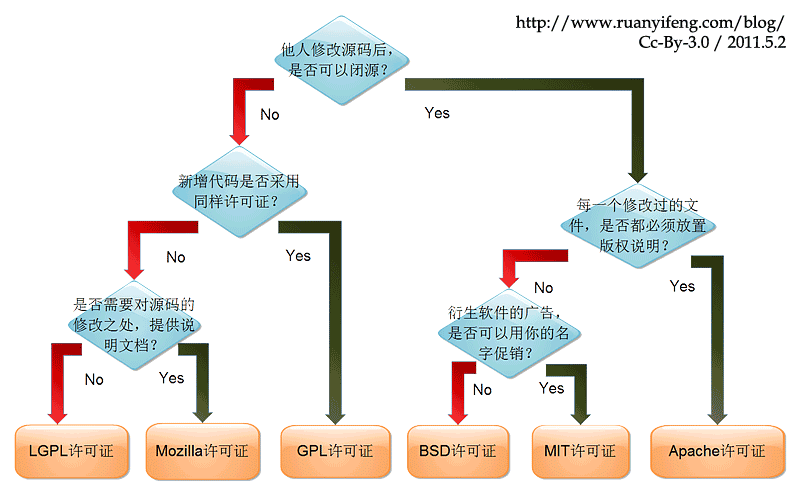
\includegraphics[width=12cm,angle=0]{figures/OpenSource.png}
%height 指定图片的高度
%width 指定图片的宽度
%angle 指定图片旋转的角度
%scale 缩放图形
\caption{Example twig query and documents }     %插入图片的标题,一般放在图片的下方,放在表格的上方
\label{fig_example1}
\end{figure}


\section{公式}
论文中的出现的公式有两种:一种是行内公式,另一种是行间居中公式。
\subsection{行内公式}
书写行内公式时只需要将公式代码放入两个\$符号中间即可,公式与行的间距将自动调整。这也是一个比Word 更方面的一个功能。比如:质能方程$E=mc^2$。
\subsection{行间公式}
书写行间方式可以将公式代码放入两个\$\$符号中间,此时无法对公式进行编号。比如:质能方程$$E=mc^2$$\par
也可以放入$\backslash$ begin\{equation\} 和 $\backslash$ end\{equation\}之间,使用此命令可以为公式进行编号,对公式进行引用等。比如:质能方程 \ref{eq1}
\begin{equation}\label{eq1}
E=mc^2
\end{equation}
